\documentclass{article}

\usepackage[brazilian]{babel}
\usepackage[a4paper,top=2cm,bottom=2cm,left=3cm,right=3cm,marginparwidth=1.75cm]{geometry}
\usepackage{amsmath}
\usepackage{array}
\usepackage{graphicx}
\usepackage[colorlinks=true, allcolors=blue]{hyperref}
\usepackage{indentfirst}

\title{Aprendizado de Máquina - Atividade Prática KNN}
\author{Willian Reichert (134090)}
\date{}

\begin{document}
\maketitle

\subsection*{Análise dos dados}

O conjunto de dados disponibilizados consiste em 30 atributos utilizados para classificar tumores de mama em malignos ou benignos, além de suas classificações as quais foram previamente realizadas. Uma breve análise que podemos fazer a respeito desses atributos é verificar qual o intervalo de valores ocupado por cada um nesse conjunto de dados, o que pode ser facilmente feito ao coletar os máximos e mínimos.

Ao observar o gráfico abaixo, o qual mostra esses intervalos, vemos que cinco atributos (X4, X5, X15, X24 e X25) se sobressaem sobre os outros, e dentro desses, dois (X5 e X25) dominam a escala de valores. Como o processo de tomada de decisão do algoritmo utiliza as distâncias entre os atributos de duas instâncias, os atributos mencionados praticamente inutilizam as contribuições dos restantes visto que eles assumem valores pequenos.

\begin{figure}[h]
    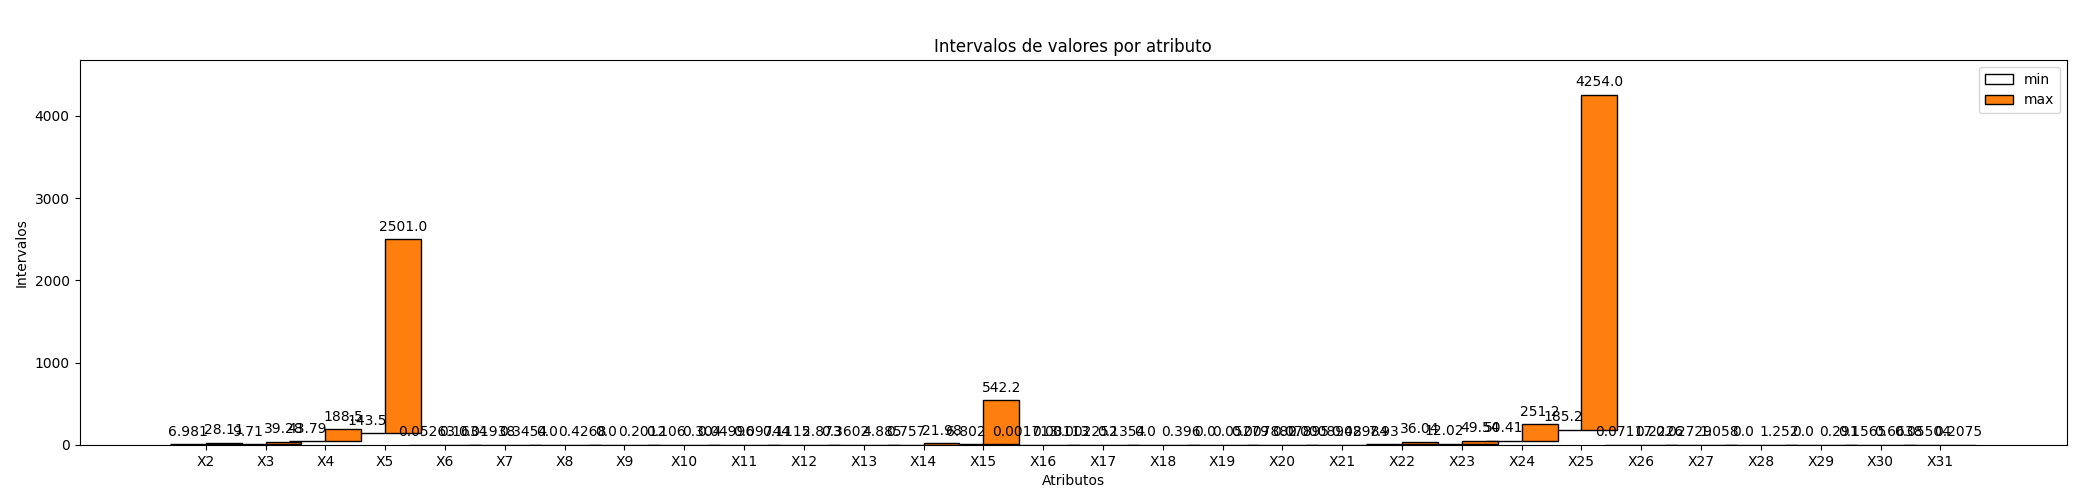
\includegraphics[width=\textwidth]{attribs_plot.png}
    \caption{Intervalos de valores por atributos presentes na base de dados}
    \centering
\end{figure}

A técnica utilizada para contornar este problema é a normalização dos dados, a qual produz valores uniformes dentro de um intervalo fixo. Neste trabalho, foi utilizada a normalização min-max [0,1], a qual iguala os pesos de cada atributo ao mapear cada escala de cada atributo para o intervalo fixo de 0 a 1.

\subsection*{Classificação sem normalização}

As classificações foram realizadas com 80\% do conjunto de dados para treino e 20\% para teste. A repartição do conjunto foi realizada com estratificação, i.e., ele foi separado em dois subconjuntos, um para cada classe, e foi coletado 20\% de cada subconjunto para compor o conjunto de testes. O restante foi atribuído para o conjunto de treinamento.

Para a classificação sem normalização foram realizadas duas coletas de dados: a primeira com apenas uma rodada do algoritmo para cada valor do hiperparâmetro \(k\) com conjuntos de treino e teste equivalentes; e a segunda com 50 repetições para cada valor de \(k\) com cada repetição tendo conjuntos de treino e teste diferentes. Apesar da distância de Manhattan ter sido implementada como uma opção, utilizou-se apenas a distância euclidiana.

\bigskip
\begin{table}[h]
\begin{center}
    \begin{tabular}{ | m{2em} | m{10em} | }
    \hline
    k & acurácia (\%) \\
    \hline
    1 & 91.304 \\
    3 & 93.913 \\
    5 & 94.783 \\
    7 & 93.913 \\
    \hline
    \end{tabular}
    \hspace{20pt}%
    \begin{tabular}{ | m{2em} | m{5em} | m{10em} | }
    \hline
    k & repetições & acurácia média (\%) \\
    \hline
    1 & 50 & 92.104 \\
    3 & 50 & 92.417 \\
    5 & 50 & 92.661 \\
    7 & 50 & 93.478 \\
    \hline
    \end{tabular}
\caption{Tabelas de dados coletados sem normalização.}
\end{center}
\end{table}

Na tabela da esquerda vemos as rodadas sem repetições. É possível notar que a acurácia melhora com o aumento do valor de \(k\) até 5, e então cai um pouco para \(k\) igual a 7. Essa queda é consequência dos conjuntos específicos de treino e teste utilizados, o que fica evidente pela acurácia média superior nesse caso quando há 50 repetições com conjuntos diferentes.

\subsection*{Classificação com normalização}

O processo utilizado nas classificações com normalização foi o mesmo de antes. Para permitir a comparação entre os valores obtidos nos testes sem repetições, os conjuntos de treino e teste utilizados foram os mesmos de antes.

\bigskip
\begin{table}[h]
\begin{center}
    \begin{tabular}{ | m{2em} | m{10em} | }
    \hline
    k & acurácia (\%) \\
    \hline
    1 & 95.652 \\
    3 & 97.391 \\
    5 & 97.391 \\
    7 & 97.391 \\
    \hline
    \end{tabular}
    \hspace{20pt}%
    \begin{tabular}{ | m{2em} | m{5em} | m{10em} | }
    \hline
    k & repetições & acurácia média (\%) \\
    \hline
    1 & 50 & 94.939 \\
    3 & 50 & 96.747 \\
    5 & 50 & 96.713 \\
    7 & 50 & 97.078 \\
    \hline
    \end{tabular}
\caption{Tabelas de dados coletados com normalização.}
\end{center}
\end{table}

Na tabela da esquerda vemos que a tendência de melhora da acurácia com o aumento do valor de \(k\) se manteve. Além disso, para essa combinação específica de conjuntos de treino e teste normalizados, as últimas três rodadas produziram a mesma quantidade de acertos. Já na tabela da esquerda verificamos, apesar da pequena queda em \(k = 5\), a tendência da acurácia aumentar até \(k = 7\), comportamento que se repete nas classificações sem normalização.

Em ambas as coletas de dados foi observado um aumento na taxa de acertos com os dados normalizados, o que era esperado visto que todos os atributos passaram a ter o mesmo peso nas tomadas de decisão.

\subsection*{Código}

O código da atividade foi enviado em um arquivo compactado. Ela foi desenvolvida com a utilização da linguagem Python, versão 3.10, e como foram utilizados apenas módulos disponibilizados com a linguagem, basta executar o arquivo \emph{KNNTester.py}, o qual contém as chamadas utilizadas para compor a coleta dos dados presentes nesse relatório.

Para utilizar o algoritmo com novos conjuntos de dados com mesmo formato, basta adicionar o arquivo csv na pasta \emph{resources} e alterar a string passada para o construtor de uma instância de um testador, \emph{TestInstance}.

\end{document}
